\section{Environtment Setup For Python}
Bahasa pemrograman python tersedia diberbagai platform, termasuk juga terdapat pada 
linux dan max os x. Untuk mengecek apakah python sudah terinstall atau belum, pertama 
tama bukalah command prompt atau terminal komputer dan ketikan python. Akan muncul info 
atau status mengenai apakah python sudah terinstall dan berapa versinya atau belum terinstall sama sekali.
  \begin{figure}[ht]
	\centerline{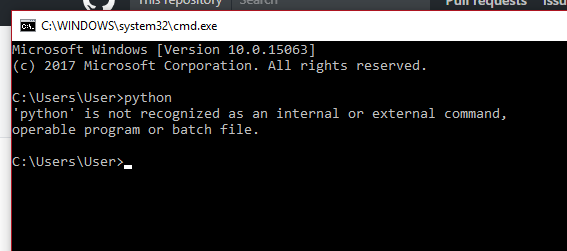
\includegraphics[width=1\textwidth]{figures/cmd.PNG}}
	\caption{Contoh skirpt pada command prompt.}
	\label{cmd}
	\end{figure}
Pada gambar \ref{cmd} memberitahukan bahwa pada komputer yang saya pakai sekarang ini belum ada atau belum terinstall python.
Ketika python belum terinstall maka sistem akan mendeteksi bahwa comand yang diberikan tidak cocok dengan yang ada disistem. 
Akan tetapi kalau sudah terinstall maka akan memunculkan nama python begitu pula versi python yang di install.
Python menyediakan dukungan yang kuat untuk integrasi dengan bahasa pemrograman lain dan alat-alat bantu lainnya. 
Python hadir dengan pustakapustaka standar yang dapat diperluas serta dapat dipelajari hanya dalam beberapa hari.
Sudah banyak programmer Python yang menyatakan bahwa mereka mendapatkan produktivitas yang lebih tinggi. 
Mereka juga merasakan bahwa Python meningkatkan kualitas 
